Evolution is change over time. Biological evolution is change over
time in the genetic composition of populations. We define the genetic
composition of a population to be the set of genomes
that the individuals in our population carry. While, at first, this definition of
evolution seems at odds with our textbook view of the evolution of
phenotypes, such as the changing shape of the finch beaks, it is genetic
changes that underpin these phenotypic changes.  \\

The genetic composition of the population can alter due to the death
of individuals or the migration of individuals in or out of the
population. If our individuals have different numbers of children,
this also alters the genetic composition of the population in the next generation. Every new individual born into the population 
subtly changes the genetic composition of the population. Their
genome is a unique combination of their parents genomes, having passed
through the process of meiosis where it is shuffled by segregation and
recombination and changed by mutation. \\

Population genetics is the study of the genetic composition of natural
populations. It seeks to understand how this composition has been changed
over time by the forces of mutation, recombination, selection,
migration, and genetic drift. 
To understand how these forces interact, it is helpful to develop simple
theoretical models to help our intuition. In these notes we will work
through these models and summarize the major areas of
population genetic theory. While these models will seem na\"{\i}ve,
and indeed they are, they are incredibly useful and powerful. 
Throughout the course we will see that these simple models yield
accurate predictions, such that much of our understanding of the
process of evolution is built on these models. We will also see how
these models are incredibly useful for understanding real patterns we
see in the evolution of phenotypes and genomes, such that much of our
analysis of evolution, in a range of areas from human genetics to
conservation, is based on these models. Therefore, population genetics is key to
understanding various applied questions from how medical genetics identifies the genes involved in
disease to how we preserve small populations (such as a Florida panther) from extinction.
\newpage

\section{Allele and genotype frequencies}
Population genetics emerged from early efforts to reconcile
Mendelian genetics with Evolution. 
Thanks to Mendel and Mendelian genetics (and a lot of prior and subsequent work), we understand that
the genome of an individual is formed from the contribution of
genomes from the gametes that fused to form zygote. The genomes of the
gametes was in turn formed from a parental genome through meiosis, in particular the segregation and
recombination of the parental genome. In this chapter we will 
work through how the basics of Mendelian Genetics play out
at the population level in sexually reproducing organisms. 
Part of the power of population genetics comes from the fact that
the rules of Mendelian genetics are very universal. Therefore, as we
build up simple models from these basic principals they are grounded
on a firm bedrock. \\

Loci and alleles are the basic currency of population genetics--and
indeed of genetics. Each individual's genetic
 makeup is defined in their genome. A \emph{locus} (plural: \emph{loci})
 is a specific spot in the genome. A locus may be an entire gene, or a single
 nucleotide base pair such as A-T. At each locus, there may be multiple genetic
 variants segregating in the population---these different genetic variants are
 known as \emph{alleles}. For example, at a particular nucleotide site in the
 genome, a population may segregate for A-T and G-C base pairs (note that due to
 the complementary nature of DNA, it will suffice to say the site segregates for
 A and G variants). If all individuals in the population carry the same allele,
 we say that the locus is \emph{monomorphic}; at this locus there is no genetic
 variability in the population. If there are multiple alleles in the population
 at a locus, we say that this locus is \emph{polymorphic}.

\subsection{Allele frequencies}

%A locus (the singular of loci) is a specific location on the genome,
%e.g. a particular DNA pair position in a gene. An allele is the genetic
%information (variant) contained at that position, for example an A-T
%base-pair. As DNA base pairs are complementary, it will suffice to say
%that there is an A allele at this locus. All of the individuals in a
%population (or a sample) may carry the same
%genetic information at this locus, in which case we will say that the%
%locus is monomorphic. Or individuals may differ in the genetic
%information they carry at a locus, for example there may be an A
%allele and a T allele at our locus. When multiple alleles are present at a locus
%the locus is said to be polymorphic.  In our example some individuals
%will be be
%homozygote for an A
%allele and some homozygote for a T allele, and some heterozygotes
%(A/T). \\


% TODO: My version, feel free to chop and incorporate Evolution is the process
% by which the genetic composition of a population changes across generations.
% Multiple forces alter the genetic composition of a population, such as
% mutation, recombination, selection, migration, and genetic drift. Population
% genetics is the study of how these forces combine to alter a population's
% genetic composition. In these notes, we summarize the major areas of
% population genetic theory that describe how these forces interact to change
% the genetic composition of a population.

% The genetic composition of a population is composed of the particular genetic
% variants the population's individuals' contain. Each individual's genetic
% makeup is defined in their \emph{genome}. A \emph{locus} (plural: \emph{loci})
% is a specific spot in the genome. A locus may be an entire gene, or a single
% nucleotide base pair such as A-T. At each locus, there may be multiple genetic
% variants segregating in the population---these different genetic variants are
% known as \emph{alleles}. For example, at a particular nucleotide site in the
% genome, a population may segregate for A-T and G-C base pairs (note that due to
% the complementary nature of DNA, it will suffice to say the site segregates for
% A and G variants). If all individuals in the population carry the same allele,
% we say that the locus is \emph{monomorphic}; at this locus there is no genetic
% variability in the population. If there are multiple alleles in the population
% at a locus, we say that this locus is \emph{polymorphic}.

Consider a diploid autosomal locus segregating at two alleles ($A_1$ and
$A_2$). We'll use these arbitrary labels for our alleles, merely to keep this
general. Let $N_{11}$ and $N_{12}$ be the number of $A_1A_1$ homozygotes and
$A_1A_2$ heterozygotes, respectively. Moreover, let $N$ be the total number of
diploid individuals in the population. We can then define the relative
frequencies of $A_1A_1$ and $A_1A_2$ genotypes as $f_{11} = N_{11}/N$ and
$f_{12} = N_{12}/N$, respectively. The frequency of allele $A_1$ in the
population is then given by

\begin{equation}
  p = \frac{2 N_{11} + N_{12}}{2N} = f_{11} + \frac{1}{2} f_{12}. 
\end{equation}

Note that this follows directly from how we count alleles given individuals'
genotypes, and holds independently of Hardy--Weinberg proportions and
equilibrium (discussed below). The frequency of the alternate allele ($A_2$) is
then just $q=1-p$.

\subsection{Hardy--Weinberg proportions}

Imagine a population mating at random with respect to genotypes, i.e. no
inbreeding, no assortative mating, no population structure, no sex differences
in allele frequencies. The frequency of allele $A_1$ in the population at the
time of reproduction is $p$. An $A_1A_1$ genotype is made by reaching out into
our population and independently drawing two $A_1$ allele gametes to form a
zygote. Therefore, the probability that an individual is an $A_1A_1$ homozygote
is $p^2$. This probability is also the expected frequency of the $A_1A_1$
homozygote in the population. The expected frequency of the three possible
genotypes is

%\begin{table}[htp!]
\begin{center}
\begin{tabular}{|ccc|}
\hline
$f_{11}$ & $f_{12}$ & $f_{22}$ \\
\hline
$p^2$ & $2pq$ & $q^2$ \\
\hline
\end{tabular}\,.
\end{center}
%\caption{\textbf{Hardy Weinberg}} \label{table:HWE}
%\end{table}
Note that we only need to assume random mating with
respect to our alleles in order for these expected frequencies to hold,
as long at $p$ is the frequency of the $A_1$ allele in the population at
the time when gametes fuse. See Figure \ref{fig:HWE_CEU_YRI} for a nice
empirical demonstration of Hardy-Weinberg proportions. 


%{\bf Q}\arabic{Question} \refstepcounter{Question} 

%\begin{question} 
%Suppose the following genotype frequencies were observed for at an esterase locus in a population of Drosophila (A denotes the “fast” allele and B denotes the “slow” allele): 
%\begin{center}
%\begin{tabular}{|ccc|}
%AA &	AB &	BB\\
%0.6 &	0.2 &	0.2\\
%\end{tabular}\,.
%\end{center}
%What genotype frequencies would you expect under Hardy Weinberg expectations?
%\end{question}

\begin{question} 
You are investigating a locus with three alleles, A, B, and C, with
allele frequencies $p_A$, $p_B$, and $p_C$. What fraction of the
population is expected to be homozygotes under Hardy-Weinberg? 
\end{question}

%%%ADD A comment about WF sampling here!
%% Also add a question about Poisson offspring number.

\begin{figure}
\begin{center}
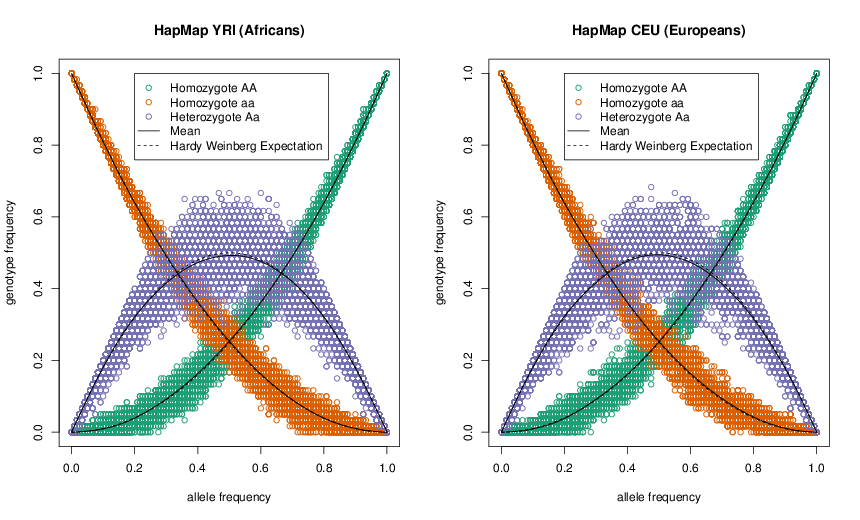
\includegraphics[width= \textwidth]{figures/CEU_YRI_separately_HWE.png}
\end{center}
\caption{Demonstrating Hardy-Weinberg proportions using 10,000 SNPs
  from the HapMap CEU European and YRI African populations. Within
  each of these populations I plot the allele frequency against the
  frequency of the 3 genotypes. Each SNP is represented by 3 different
  coloured points. The solid lines show the mean genotype frequency
  (calculated using a loess smoothing). The dashed line shows the
  predicted genotype frequency from Hardy Weinberg equilibrium. I find
  it really pretty that the analytical predictions work as well as
  they do. See \href{blog post}{http://gcbias.org/2011/10/13/population-genetics-course-resources-hardy-weinberg-eq/} here on this plot. } \label{fig:HWE_CEU_YRI}
\end{figure}


%\begin{figure}
%\begin{center}
%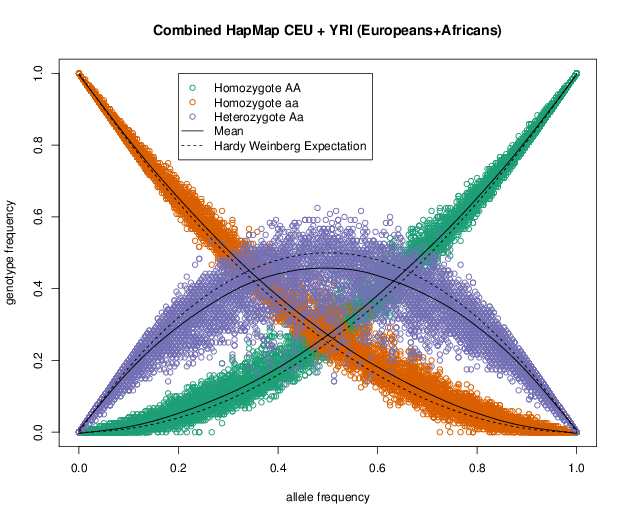
\includegraphics[width=0.5 \textwidth]{figures/CEU_YRI_together_HWE.png}
%\end{center}
%\caption{}
%\end{figure}


%figure/QT1.eps


\subsection{Allele sharing among related individuals and Identity by Descent}

% TODO: VB added some stuff here
All of the individuals in a population are related to each other by a giant
pedigree (family tree). For most pairs of individuals in a population these
relationships are very distant (i.e. distant cousins), while some individuals
will be more closely related (i.e. sibling/first cousins). All individuals of
are related to one another by varying levels of relatedness, or \emph{kinship}.
Related individuals can share alleles that have both descended from the shared
common ancestor. To be shared, these alleles must be inherited through all
meioses connecting the two individuals (e.g. surviving the $\nicefrac{1}{2}$
probability of segregation each meiosis). As fewer closer relatives are
separated by fewer meioses, closer relatives share more alleles. In Figure
\ref{fig:IBD_cousins_chr_cartoon} we show the sharing of chromosomal regions
between two cousins. As we are interested in the genetics of populations we are
interested in kinship, and so we need some way to quantify the degree of
kinship among individuals.\\ 

\begin{figure}
\begin{center}
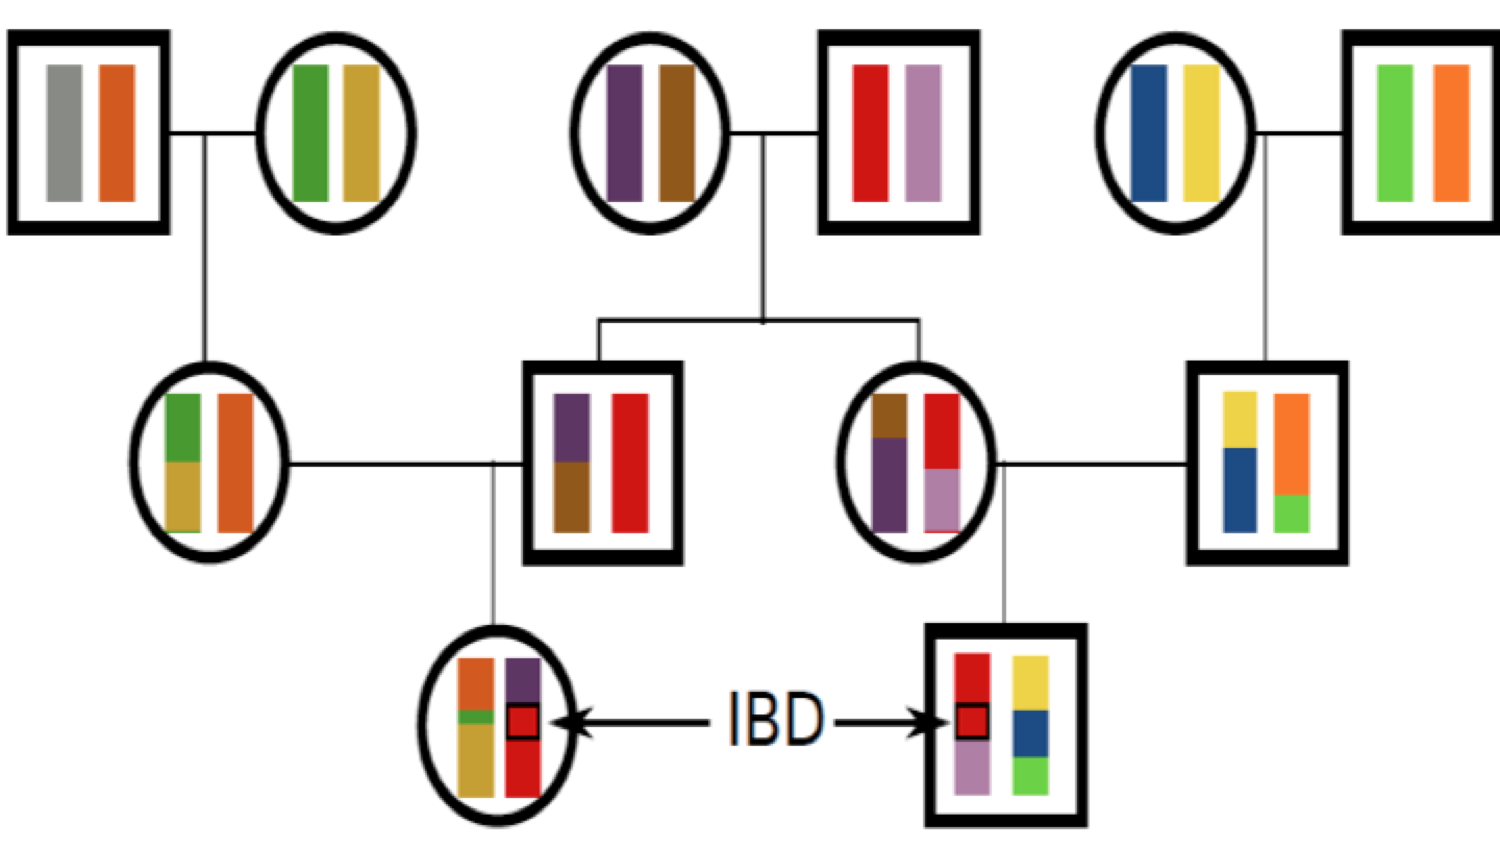
\includegraphics[width= 0.5 \textwidth]{figures/Cousins_IBD_chromo_cartoon.png}
\end{center}
\caption{First cousins sharing a stretch of chromosome identical by
  descent. The different grandparental diploid chromosomes are coloured so we
  can track them and recombinations between them across the
  generations. Notice that the identity by descent between the cousins persists for a long
stretch of chromosome due to the limited number of generations for
recombination.} \label{fig:IBD_cousins_chr_cartoon}  
\end{figure}

We will define two alleles to be identical by descent (IBD) if they are
identical due to a common ancestor in the past few generations. For the moment,
we ignore mutation, and we will be more precise about what we mean by `past few
generations' later on. For example, parent and child share exactly one allele
identical by descent at a locus, assuming that the two parents of the child are
randomly mated individuals from the population. In Figure
\ref{fig:IBD_cousins_cartoon} I show a pedigree demonstrating some
configurations of IBD. \\


A key quantity is the probability that our pair of individuals share
0, 1, or 2 alleles identical by descent (see Figure \ref{fig:IBD_0_1_2}). We denote these probabilities
by $r_0$, $r_1$, and $r_2$ respectively. See Table \ref{table:IBDprobs} for
some examples. We can also interpret these probabilities as
genome-wide averages. For example, on average, full-sibs share zero alleles for a
quarter of all of their autosomal loci.\\

\begin{figure}
\begin{center}
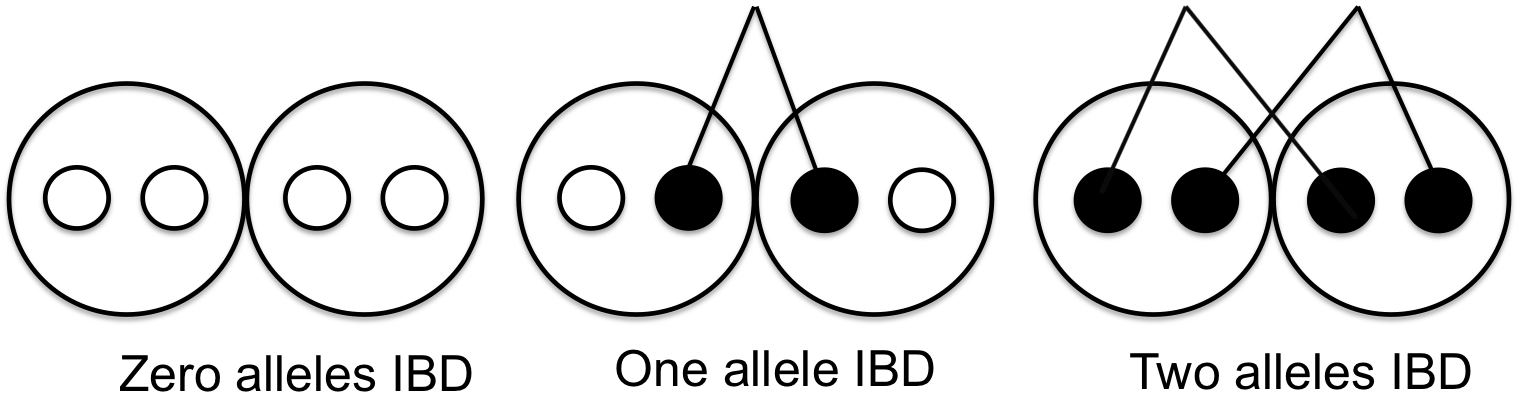
\includegraphics[width= \textwidth]{figures/IBD_0_1_2.png}
\end{center}
\caption{Three pairs of diploid individuals sharing 0, 1, or 2 alleles IBD
  where lines show the sharing of alleles by descent (e.g. from a
  shared ancestor). } \label{fig:IBD_0_1_2}
\end{figure}

\begin{figure}
\begin{center}
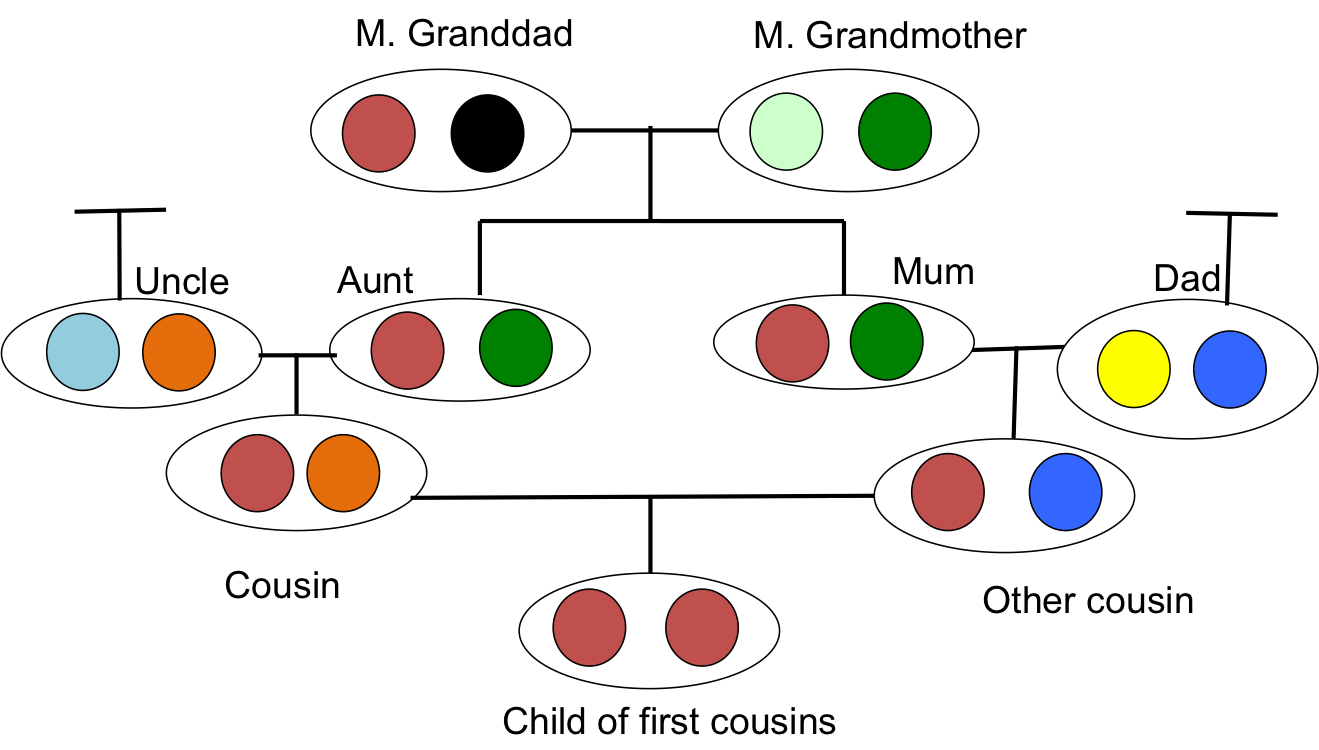
\includegraphics[width= 0.5 \textwidth]{figures/Child_first_cousins_Homozy_BD.png}
\end{center}
\caption{Alleles being transmitted through an inbred pedigree. The mum and the
  aunt share two alleles identical by descent (IBD). The cousins share one
  allele IBD. The offspring of first cousins is homozygous by
  descent at this locus.} \label{fig:IBD_cousins_cartoon}  
\end{figure}


One summary of relatedness that will be important is the probability that two alleles picked at random, one from each of the two different individuals $i$ and $j$, are identical by descent. We call this quantity the coefficient of kinship of individuals $i$ and $j$, and denote it by $F_{ij}$. It is calculated as
\begin{equation}
F_{ij}= 0 \times r_0 + \frac{1}{4} r_1  + \frac{1}{2} r_2. 
\label{eqn:coeffkinship}
\end{equation}

The coefficient of kinship will appear multiple times, in both our discussion of
inbreeding and in the context of phenotypic resemblance between relatives.\\

\begin{table}
\begin{center}
\begin{tabular}{| l | c c c c|}
\hline
Relationship (i,j)$^{*}$ & $r_0$ & $r_1$ & $r_2$ & $F_{ij}$\\
\hline
parent--child & 0 & 1 & 0 & 1/4\\
full siblings & 1/4 & 1/2 & 1/4 & 1/4\\
identical (monzygotic) twins  & 0 & 0 & 1  & 1/2 \\
$1^{st}$ cousins & 3/4 & 1/4 & 0 & 1/16\\
\hline
\end{tabular}
\end{center}
\caption{Probability that two individuals of a given relationship share 0, 1, or 2 alleles
identical by descent on the autosomes. $^{*}$ assuming this is the only relationship
the pair of individuals share (above that expected from randomly
sampling individuals from the population). } \label{table:IBDprobs}
\end{table}

\begin{question}
What are $r_0$, $r_1$, and $r_2$ for 1/2 sibs? (1/2 sibs share one
parent but not the other).
\end{question}

%{\bf Q}\arabic{Question} \refstepcounter{Question} 
\begin{question} 
Consider a biallelic locus where allele 1 is
at frequency $p$, and two individuals who have IBD allele sharing
probabilities $r_0$, $r_1$, $r_2$. \\
What is the overall probability that these
two individuals are both homozygous for allele 1?\\
%{\bf} What is the probability that both individuals heterozygotes? 
\end{question}



\subsection{Inbreeding}
We can define an inbred individual as an individual whose parents are
more closely related to each other than two random individuals drawn
from some reference population.  \\

When two related individuals produce an offspring, that individual can
receive two alleles that are identical by descent, i.e.\ they
can be homozygous by descent (sometimes termed autozygous), due to the
fact that they have two copies of an allele through different paths
through the pedigree.  This increased likelihood of being homozygous
relative to an outbred individual is the most obvious effect of
inbreeding. It is also the one that will be of most interest to us, as it
underlies a lot of our ideas about inbreeding depression and
population structure. For example, in figure \ref{fig:IBD_cousins_cartoon} our
offspring of first cousins is homozygous by descent having received
the same IBD allele via two different routes around an inbreeding loop.\\

As the offspring receives a random allele from each parent ($i$ and $j$), the
probability that those two alleles are identical by descent is equal to the
kinship coefficient $F_{ij}$ of the two parents (Eqn.\ \ref{eqn:coeffkinship}). This follows from the fact that
the genotype of the offspring is made by sampling an allele at random from each
of our parents. We will use IBD for identical by descent. \\

The only way the offspring can be heterozygous ($A_1 A_2$) is if their two alleles at a
locus are not IBD (otherwise they would necessarily be homozygous). Therefore, the probability that they are
heterozygous is
\begin{equation}
(1-F) 2p q,
\label{eq:hetGenHW}
\end{equation}
where we have dropped the indices $i$ and $j$ for simplicity.
The offspring can be homozygous for the $A_1$ allele in two different ways. 
They can have two non-IBD alleles that are not IBD but happen to be of the allelic type $A_1$,
or their two alleles can be IBD, such that they inherited allele $A_1$ by
two different routes from the same ancestor. Thus, the probability that an offspring is homozygous is
\begin{equation}
(1-F) p^2 + F p.
\end{equation}
Therefore, the frequencies of the three possible genotypes can be written as given in
Table \ref{table:GeneralizedHWE}, which provides a generalization of the Hardy--Weinberg
proportions.\\

\begin{table}
\begin{center}
\begin{tabular}{|ccc|}
\hline
$f_{11}$ & $f_{12}$ & $f_{22}$ \\
\hline
$(1-F) p^2 + F p$ & $(1-F) 2pq$ & $(1-F) q^2 + F q$ \\
\hline
\end{tabular}
\end{center}
\caption{\textbf{Generalized Hardy--Weinberg}} \label{table:GeneralizedHWE}
\end{table}

Note that the generalized Hardy--Weinberg proportions completely
specify the genotype probabilities, as there are two parameters ($p$ and $F$)
and two degrees of freedom (as $p$ and $q$ have to sum to one).
Therefore, any combination of genotype frequencies at a biallelic site
can be specified by a combination of $p$ and $F$.\\

\begin{question}
The frequency of the $A_1$ allele is p the frequency of the $A_2$ allele is q. Assume that our population is randomly mating and that the genotype frequencies in the population follow from HW. We select two individuals at random to mate from this population. We then mate the children from this cross. What is the probability that the child from this sib-mating is homozygous? 
\end{question}

\subsection{Calculating inbreeding coefficients from data}
If the observed heterozygosity in a population is $H_O$, and we assume that the generalized Hardy--Weinberg proportions hold, we can set $H_O$ equal to $f_{12}$, and solve Eq.\ \eqref{eq:hetGenHW} for $F$ to obtain an estimate of the inbreeding coefficient as
\begin{equation}
\hat{F} = 1-\frac{f_{12}}{2pq} = \frac{2pq - f_{12}}{2pq}.
\label{eqn:Fhat}
\end{equation}
As before, $p$ is the frequency of allele $A_{1}$ in the
population. This can be rewritten in terms of the observed heterozygosity ($H_O$)
and the heterozygosity expected in the absence of inbreeding, $H_E=2pq$, as
\begin{equation}
\hat{F} = \frac{H_E-H_O}{H_E} = 1 - \frac{H_O}{H_E}.
\label{eqn:FhatHO}
\end{equation}
Hence, $\hat{F}$ quantifies the deviation due to inbreeding of the observed heterozygosity from the one expected under random mating, relative to the latter.
If we have multiple loci, we can replace $H_O$ and $H_E$ by their means
over loci, $\bar{H}_O$ and $\bar{H}_E$, respectively. Note that, in principle, we could also calculate $F$ for each individual locus first, and then take the average across loci. However, this procedure is more prone to introducing a bias if sample sizes vary across loci, which is not unlikely when we are dealing with real data.\\

%{\bf Q}\arabic{Question} \refstepcounter{Question} 
\begin{question} 
Suppose the following genotype frequencies were observed for at an esterase locus in a population of Drosophila (A denotes the “fast” allele and B denotes the “slow” allele): 
\begin{center}
\begin{tabular}{|ccc|}
AA &	AB &	BB\\
0.6 &	0.2 &	0.2\\
\end{tabular}\,.
\end{center}
What is the estimate of the inbreeding coefficient at the esterase locus?
\end{question}

%==Phenotypic resemblance between relatives ==
%<source-file filename="Quantative_traits.tex" display="Quantative_traits.wrapped.latexml.xhtml">

%==Phenotypic resemblance between relatives ==
%<source-file filename="Quantative_traits.tex" display="Quantative_traits.wrapped.latexml.xhtml">


\subsection{Summarizing population structure}
We defined inbreeding as having parents that are
more closely related to each other than two individuals drawn at random from some reference population. The question that naturally arises is: Which reference population should we use? While I might not look inbred in
comparison to allele frequencies in the United Kingdom (UK), where I am from, my
parents certainly are not two individuals drawn at random from the
world-wide population. If we estimated my inbreeding coefficient $F$ using allele frequencies
within the UK, it would 
be close to zero, but would likely be larger if we used world-wide
frequencies. This is because there is a somewhat lower level of
expected heterozygosity within the UK than in the human population across the world as a whole.\\

Wright (1943, 1951) developed a set of `F-statistics' (also called `fixation indices') that formalize the idea
of inbreeding with respect to different levels of population
structure. See figure \ref{fig:FST_pig} for a schematic diagram. He defined $F_{\mathrm{XY}}$ as
the correlation between random gametes, drawn from the same level $X$,
relative to level $Y$. We will return to why $F$-statistics are statements
about correlations between alleles in just a moment. One commonly uses $\fis$ for the inbreeding
coefficient between an individual ($I$) and the subpopulation
($S$). Consider a single locus, where in a subpopulation ($S$) a fraction $H_I=f_{12}$ of individuals
are heterozygous. In this subpopulation, let the frequency of
allele $A_1$ be $p_S$, such that the expected heterozygosity under random mating is $H_S = 2 p_S (1 - p_S)$. We will write $\fis$ as
\begin{equation}
\fis = 1-\frac{H_I}{H_S}= 1-\frac{f_{12}}{2p_Sq_S},
\label{eqn:FIS}
\end{equation}
a direct analog of eqn. \ref{eqn:Fhat}. Hence, $\fis$ is the relative difference between observed and expected heterozygosity due to a deviation from random mating within the subpopulation. We could also compare the observed
heterozygosity in individuals ($H_I$) to that expected in the total
population, $H_T$. If the frequency of allele $A_1$ in the total
population is $p_T$, then we can write $\fit$ as
\begin{equation}
\fit =1-\frac{H_I}{H_T}= 1-\frac{f_{12}}{2p_Tq_T},
\label{eqn:FIT}
\end{equation}
which compares heterozygosity in individuals to that expected in the
total population. As a simple extension of this, we could imagine
comparing the expected heterozygosity in the subpopulation ($H_S$) to
that expected in the total population $H_T$, via $\fst$:
\begin{equation}
\fst = 1-\frac{H_S}{H_T}=1-\frac{2p_Sq_S}{2p_Tq_T} \label{eqn:FST}.
\end{equation}
If the total population contains the subpopulation then
 $2p_Sq_S \leq
2p_Tq_T$, and so $\fis \leq \fit$ and $\fst \geq 0$. We can
relate the three $F$-statistics to each other as
\begin{equation}
(1-\fit) =\frac{H_I}{H_S} \frac{H_S}{H_T}=(1-\fis)(1-\fst).
\label{eqn:F_relationships}
\end{equation}
Hence, the reduction in heterozygosity within individuals compared to that expected
in the total population can be decomposed to the reduction in
heterozygosity of individuals compared to the subpopulation, and the reduction in
heterozygosity from the total population to that in the subpopulation.\\
%n, as we will seebelow, due to the Wahlund effect (to be added)
\begin{figure}
\begin{center}
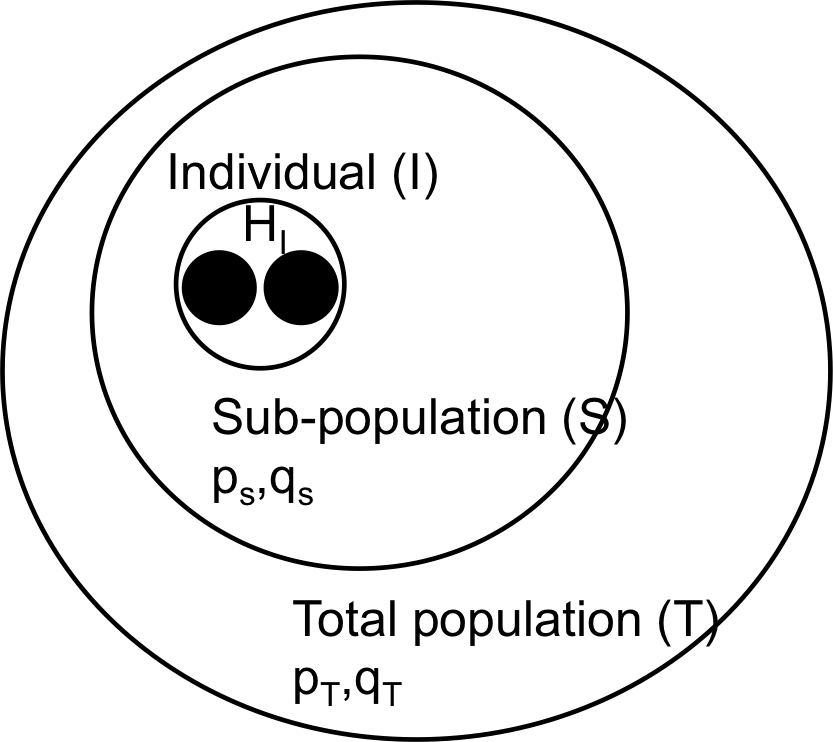
\includegraphics[width= 0.5 \textwidth]{figures/FST_pig.png}
\end{center}
\caption{A diagram showing the hierarchical nature of F
  statistics. The two solid dots within an individual show the two
  alleles at a locus for an individual $I$. We
  can compare the heterozygosity on individuals ($H_i$), to that found
by randomly drawing alleles from the sub-population ($H_S=2p_Sq_S$),
to that found in the total population ($H_T=2p_Tq_T$). } \label{fig:FST_pig}  
\end{figure}

If we want a summary of
population structure across multiple subpopulations, we can average $H_I$
and/or $H_S$ across populations, and use a $p_T$ calculated by
averaging $p_S$ across subpopulations (or our samples from sub-populations). For example, the average $\fst$ across $K$ subpopulations (sampled with equal effort) is
\begin{equation}
	\fst = 1 - \frac{\bar{H}_{S}}{H_T},
\end{equation}
where $\bar{H}_S = 1/K \sum_{i = 1}^{K} H_{S}^{(i)}$, and $H_{S}^{(i)} = 2 p_{i} q_{i}$ is the expected heterozygosity in subpopulation $i$.
Furthermore, if we have multiple sites, we can replace $H_I$, $H_S$, and $H_T$ with their averages across loci (as above). \\

\paragraph{Interpretations of F-statistics.}
Let us now return to Wright's definition of the $F$-statistics as correlations between random gametes, drawn from the same level $X$,
relative to level $Y$. Without loss of generality, we may think about $X$ as
individuals and $S$ as the subpopulation.
Rewriting $\fis$ in terms of the observed homozygote frequencies ($f_{11}$, $f_{22}$) and expected homozygosities ($p_{S}^2$, $q_{S}^2$) we find
\begin{equation}
\fis = \frac{2p_Sq_S - f_{12}}{2p_Sq_S} = \frac{f_{11}+f_{22} -
p_S^2 - q_S^2}{2p_Sq_S},
\label{eqn:Fascorr}
\end{equation}
using the fact that $p^2+2pq+q^2=1$, and $f_{12} = 1 - f_{11} - f_{12}$. The form of eqn.\ (\ref{eqn:Fascorr}) reveals that $\fis$ is the covariance between pairs of alleles
found in an individual, divided by the
expected variance under binomial sampling. Thus, $F$-statistics can be
understood as the correlation between alleles drawn from a population
(or an individual) above that expected by chance (i.e.\ drawing alleles
sampled at random from some broader population).\\

We can also interpret $F$-statistics as proportions of variance explained by
different levels of population structure. To see this, let us think about $\fst$ averaged over $K$
subpopulations, whose frequencies are $p_1,\dots,p_K$. The
frequency in the total population is $p_T=\bar{p} = 1/K \sum_{i=1}^K p_i$.
Then, we can
write
\begin{equation}
\fst = \frac{2 \bar{p}\bar{q} - \frac{1}{K}\sum_{i=1}^K 2p_iq_i }{2
\bar{p}\bar{q}} = \frac{ \left(\frac{1}{K} \sum_{i=1}^K p_i^2 +
\frac{1}{K} \sum_{i=1}^K q_i^2 \right) -  \bar{p}^2-\bar{q}^2 }{2
\bar{p}\bar{q}} = \frac{\mathrm{Var}(p_i)}{\mathrm{Var}(\bar{p})},
\label{eqn:F_as_propvar}
\end{equation}
which shows that $\fst$ is the proportion of the variance explained by the
subpopulation labels.

\subsection{Other approaches to population structure}
There is a broad spectrum of methods to describe patterns of
population structure in populaion genetic datasets. We'll briefly
discuss two broad-classes of methods, assigment methods and principal
components analysis,that appear often in the literature.

\subsubsection{Assignment Methods}

Here we'll describe a simple probabilistic assignment to find the
probability that an individual of unknown population comes from one of
$K$ predefined populations. We'll then briefly explain how to extend this
to cluster individuals into $K$ initially unknown populations. This
method is a simplified version of what Bayesian population genetics
clustering algorithms such as STRUCTURE and ADMIXTURE do (Pritchard et al. Genetics 2000). 

\paragraph{A simple assignment method}

We have genotype data from unlinked S bi-allelic loci for $K$ populations. The allele frequency of allele $A_1$ at locus $l$ in population $k$ is denoted by $p_{k,l}$, so that the allele frequencies in population 1 are $p_{1,1},\cdots p_{1,L}$ and population 2 are $p_{2,1},\cdots p_{2,L}$ and so on. 

You type a new individual from an unknown population at these $L$ loci. This individual's genotype at locus $l$ is $g_l$, where $g_l$ denotes the number of copies of allele $A_1$ this individual carries at this locus ($g_l=0,1,2$). 

The probability of this individual's genotype at locus $l$ conditional on coming from population $k$ (i.e. their alleles being a random HW draw from population $k$) is 
\begin{equation}
P(g_l | \textrm{pop k}) = I(g_l=0) (1-p_{k,l})^2 +  I(g_l=1) 2 p_{k,l} (1-p_{k,l}) + I(g_l=2) p_{k,l}^2
\end{equation}
where $I(g_l=0)$ is an indicator function which is $1$ if $g_l=0$ and
zero otherwise, and likewise for the other indicator functions. This
follows simply from HWE.

Assuming that the loci are independent, the probability of individual's genotypes conditional on them coming from population $k$ is 
\begin{equation}
P(\textrm{ind.} | \textrm{pop k})  = \prod_{l=1}^S P(g_l | \textrm{pop k}) \label{eqn_assignment}
\end{equation}

We wish to know the probability that this new individual comes from population $k$, i.e. $P(\textrm{pop k} | \textrm{new ind.})$. We can obtain this through Bayes rule 
\begin{equation}
 P(\textrm{pop k} | \textrm{ind.})  = \frac{P(\textrm{ind.} | \textrm{pop k}) P(\textrm{pop k})}{P(\textrm{ind.})}
\end{equation}
where 
\begin{equation}
P(\textrm{ind.}) = \sum_{k=1}^K  P(\textrm{ind.} | \textrm{pop k}) P(\textrm{pop k})
\end{equation}
is the normalizing constant. We interpret $P(\textrm{pop k})$ as the
prior probability of the individual coming from population $k$, unless
we have some other prior knowledge we will assume that the new individual has a equal probability of coming from each population $P(\textrm{pop k})=1/K$.  

We intepret 
\begin{equation}
 P(\textrm{pop k} | \textrm{ind.})
\end{equation}
as the posterior probability that our new individual comes from each of our $1,\cdots, K$ populations.

More sophisticated versions of this are now used to allow for hybrids,
e.g, we can have a proportion $q_k$ of our individual's genome come
from population $k$ and estimate the set of $q_k$'s.

%{\bf Q}\arabic{Question} \refstepcounter{Question}  
\begin{question} 
We have two populations where the frequency of capital allele
at two SNPs ($A/a$ and $B/b$)  is given by
\begin{center}
\begin{tabular}{|ccc|}
\hline
Population & locus A & locus B \\
\hline
1 & $0.1$ & $0.85$ \\
2  & $0.95$ & $0.2$ \\
\hline
\end{tabular}
\end{center}
We sample an individual whose genotype is $AA$ at the first locus
and $bb$ at the second. What
is the posterior probability that our indvidual comes from population 1 vs
population 2?
Lets assume that with probability $q_1$ our individual draws an allele
from population $1$ and that with probability $q_2=1-q_1$ they draw an allele from
population $2$. What is the probability of our individual's genotype
given $q_1$? You could plot this probability as a function of $q_1$. How does 
your plot change if our individual is heterozygote at both loci?
\end{question} 

\paragraph{Clustering based on assignment methods}
While it is great to be able to assign our individuals to particular
population, these ideas can be pushed to learn about how best to
describe our genotype data in terms of discrete populations without
assigning any of our individuals to populations {\it a priori}. 
We wish to cluster our individuals into $K$ unknown populations. We begin by assigning our individuals at random to these $K$ populations. 
\begin{itemize}
\item Given these assignments we estimate the allele frequencies at all of our loci in each population. 
\item Given these allele frequencies we chose to reassign each individual to a population $k$ with a probability given by eqn. ($\ref{eqn_assignment}$).
\end{itemize}
We iterate steps 1 and 2 for many iterations. If the data is sufficiently informative the assignments and allele frequencies will quickly converge. 

To do this in a full bayesian scheme we need to place priors on the
allele frequencies (e.g. a beta distribution).Technically we are using
this is the joint posterior of our allele frequencies and assignments. 

\subsubsection{Principal components analysis}
The use of principal component analysis in population genetics was
pioneered by Cavalli-Sforza. With large genotyping datasets PCA has made
a come back. See Patterson et al 2006, PLoS Genetics and McVean,
G. 2010 PLoS Genetics and for recent discussion.
 
Consider a dataset consisting of N individuals at S bi-allelic
SNPs. The $i^{th}$ individual's genotype data at locus $\ell$ takes
value $g_{i,\ell}$=0,1, or 2 (corresponding to the number of copies of
allele $A_1$ an individual carrys at this SNP). We can think of this
as a N x S matrix (where usually $N \ll S$). 

 Denoting the sample mean allele freq at SNP $\ell$ by $p_{\ell}$ we usually standardize the genotype in the following way
\begin{equation}
\frac{g_{i,\ell} - 2 p_{\ell}}{\sqrt{p_{\ell}(1-p_{\ell})}}
\end{equation}
i.e. at each SNP we center the genotypes by minusing of the mean
genotype ($2\epsilon_{\ell}$) and divide through by the expected
variance assuming that alleles are sampled binomially from the mean
frequency ($\sqrt{p_{\ell} (1-p_{\ell})}$). Doing this to
all of our genotypes we form a data matrix (of dimension N x S). We
can then perform principal components analysis of this data matrix to
cover the major axes of genotype variance in our sample.

It is worth taking a moment to delve further into what we are doing
here. There's a number of equivalent ways to thinking about what PCA
is doing, one of these is to think that when we do PCA we are building the individual by individual
covariance matrix and performing eigen-value decomposition of this
matrix (with the eigen-vectors giving the PC).  This individual by individual covariance matrix has entries
the $(i,~j)^{th}$ entry given by
\begin{equation}
\sum_{\ell=1}^S \frac{(g_{i,\ell} - 2p_{\ell})(g_{j,\ell} - 2p_{\ell})}{p_{\ell}(1-p_{\ell})}
\end{equation}
note that this is the covariance, is very similar to those we
encountered in discussing $F$-statistics as correlations (equation
\eqref{eqn:Fascorr}), expect now we are asking about the allelic covariance
between two individuals above that expected if they were both drawn
from the total sample at random (rather than the covariance of alleles
within a single individual). So by performing PCA on the data we are
learning about the major (orthogonal) axes of the kinship matrix.    


\newpage
\subsection{Correlations between loci, linkage disequilibrium, and recombination}

%</source-file>

Up to now we have been interested in correlations between alleles at the
same locus, e.g. correlations within individuals (inbreeding) or between
individuals (relatedness). We have seen how relatedness between parents affects the extent to which their offspring is inbred. We now turn to 
correlations between alleles at different loci. To understand
correlations between loci we need to understand recombination.\\


\paragraph{Recombination}  Lets
consider an individual heterozygous for a $AB$ and $ab$
haplotype. If no recombination occurs between our two loci in this
individual, then these two haplotypes will be transmitted intact to
the next generation. While if a recombination (or more generally an
odd number of recombinations) occurs between our two loci on the
haplotype transmitted to the child then $\tfrac{1}{2}$ the time the
child receives a $Ab$ haplotype and $\tfrac{1}{2}$ the time the child
receives a $aB$ haplotype. So recombination is breaking up the
association between loci. We'll define the recombination fraction ($r$) to be
the probability of an odd number of recombinations between our loci.
In practice we'll often be interested in relatively short regions
where recombination is relatively rare, and so we might think that
$r=r_{BP}L \ll 1$, where $r_{BP}$ is the average recombination rate
per base pair (typically $\sim 10^{-8}$) and L is the number of base
pairs separating our two loci.\\



\paragraph{Linkage disequilibrium}
The (horrible) phrase linkage
disequilibrium (LD) refers to the statistical non-independence
(i.e. a correlation)  of
alleles at different loci. Our two loci, which segregate alleles $A/a$ and $B/b$, have allele
frequencies of $p_A$ and $p_B$ respectively. The frequency of the two locus haplotype is $p_{AB}$,
and likewise for our other three combinations. If our loci were
statistically independent then $p_{AB} = p_Ap_B$, otherwise $p_{AB} \neq p_Ap_B$
We can define a covariance between the $A$ and $B$ alleles at our two loci as
\begin{equation}
D_{AB} = p_{AB} - p_Ap_B
\end{equation}
and likewise for our other combinations at our two loci
($D_{Ab},~D_{aB},~D_{ab}$). These $D$ statistics are all closely
related to each other as $D_{AB} = - D_{Ab}$ and so on. Thus we only
need to specify one $D_{AB}$ to know them all, so we'll drop the
subscript and just refer to $D$. Also a handy result is that we can rewrite our haplotype
frequency $p_{AB}$ as
\begin{equation}
p_{AB} = p_Ap_B+D. \label{eqn:ABviaD}
\end{equation}
If $D=0$ we'll say the two loci are in linkage equilibrium, while if
$D>0$ or $D<0$ we'll say that the loci are in linkage
disequilibrium (we'll perhaps want to test whether $D$ is
statistically different from $0$ before making this choice). You should be careful to keep the concepts of linkage
and linkage disequilibrium separate in your mind. Genetic linkage refers to the
linkage of multiple loci due to the fact that they
are transmitted through meiosis together (most often because the
loci are on the same chromosome). Linkage disequilibrium merely refers
to the correlation between the alleles at different loci, this may in
part be due to the genetic linkage of these loci but does not
necessarily imply this (e.g. genetically unlinked loci can be in LD
due to population structure). \\

Another common statistic for summarizing LD is $r^2$ which we write as
\begin{equation}
r^2 = \frac{D^2}{p_A(1-p_A) p_B(1-p_B) }
\end{equation}
as $D$ is a covariance, and $p_A(1-p_A) $ is the variance of an allele
drawn at random from locus $A$, $r^2$ is the squared correlation
coefficient.    \\

%{\bf Q}\arabic{Question} \refstepcounter{Question}  
\begin{question} 
You genotype 2 bi-allelic loci (A \& B) segregating in two mouse subspecies (1 \& 2) which mate randomly among themselves, but have not historically interbreed since they speciated. On the basis of previous work you estimate that the two loci are separated by a recombination fraction of 0.1. The frequencies of haplotypes in each population are:
\begin{center}
\begin{tabular}{|c|cccc|}
\hline
Pop    & $p_{AB}$    & $p_{Ab}$ &    $p_{aB}$ &    $p_{ab}$\\
\hline
1 &    .02    & .18 &     .08 &    .72\\
2&    .72 &    .18 &    .08 &    .02\\
\hline
\end{tabular}
\end{center}

{\bf A)} How much LD is there within populations, i.e. estimate D?\\

{\bf B)} If we mixed the two populations together in equal proportions what value would D take before any mating has had the chance to occur? \\
\end{question}


\paragraph{The decay of LD due to recombination}
We will now examine what happens to LD over the generations if we
only allow recombination to occur in a very large population (i.e. no
genetic drift, i.e. the frequencies of our loci follow their expectations). To do so consider the frequency of our $AB$ haplotype in the next generation
$p_{AB}^{\prime}$. We lose a fraction $r$ of our $AB$ haplotypes to
recombination ripping our alleles apart but gain a fraction $rp_A p_B$ per generation from other
haplotypes recombining together to form $AB$ haplotypes. Thus in the
next generation
\begin{equation}
p_{AB}^{\prime} = (1-r)p_{AB} + rp_Ap_B
\end{equation}
this last term here is $r(p_{AB}+p_{Ab})(p_{AB}+p_{aB})$, which
multiplying this out is the
probability of recombination in the different diploid genotypes that
could generate a $p_{AB}$ haplotype. \\

We can then write the change in the frequency of the $p_{AB}$
haplotype as
\begin{equation}
\Delta p_{AB} = p_{AB}^{\prime} -p_{AB} = -r p_{AB} + rp_Ap_B = - r D
\end{equation}
so recombination will cause a decrease in the frequency of $p_{AB}$ if
there is an excess of $AB$ haplotypes within the population ($D>0$), and an
increase if there is a deficit of $AB$ haplotypes within the
population ($D<0$). Our LD in the next generation is $D^{\prime} =
p_{AB}^{\prime}$, so we can rewrite the above eqn. in terms of the
$D^{\prime} $
\begin{equation}
D^{\prime}= (1-r) D
\end{equation}
so if the level of LD in generation $0$ is $D_0$ the level $t$
generations later ($D_t$) is
\begin{equation}
D_t=  (1-r)^t D_0
\end{equation}
so recombination is acting to decrease LD, and it does so
geometrically at a rate given by $(1-r)$. If $r \ll 1$ then we can
approximate this by an exponential and say that   
\begin{equation}
D_t \approx  D_0 e^{-rt}
\end{equation}\\



%{\bf Q}\arabic{Question} \refstepcounter{Question}  
\begin{question} 
You find a hybrid population between the two mouse subspecies
described in the question above, which appears to be comprised of equal proportions of ancestry from the two subspecies.  You estimate LD between the two markers to be 0.0723. Assuming that this hybrid population is large and was formed by a single mixture event, can you estimate how long ago this population formed? \\
\end{question}
%\subsection{Testing for departures from HWE.}
%Note the form of $\hat{F}$ \eqref{eqn:FhatHO} is the same as the $X^2$
%statistic, and so we can test for a deviation from hardy-weinberg  $X^2$


%\subsection{Population structure}
%The question naturally arises at this point: what reference population
%(i.e. what allele frequency) do we use to calculate $\hat{F}$? If we are %calculating the inbreeding coefficient
%of an English person do we use the frequencies of the town of that
%person, of England, of the United Kingdom, or of the World?



%\gc{Include the HapMap exercise here?}


%==One locus models of selection==
%<source-file filename="one_loc_sel_models.tex" display="one_loc_sel_models.wrapped.latexml.xhtml">

\newpage

